\documentclass[a4paper]{article}
\usepackage{vntex}
%\usepackage[english,vietnam]{babel}
%\usepackage[utf8]{inputenc}

%\usepackage[utf8]{inputenc}
%\usepackage[francais]{babel}
\usepackage{a4wide,amssymb,epsfig,latexsym,multicol,array,hhline,fancyhdr}

\usepackage{amsmath}
\usepackage{lastpage}
\usepackage[lined,boxed,commentsnumbered]{algorithm2e}
\usepackage{enumerate}
\usepackage{listings}
\usepackage{color}
\usepackage{graphicx}							% Standard graphics package
\usepackage{array}
\usepackage{tabularx, caption}
\usepackage{subcaption}
\usepackage{multirow}
\usepackage{multicol}
\usepackage{rotating}
\usepackage{graphics}
\usepackage{geometry}
\usepackage{setspace}
\usepackage{epsfig}
\usepackage{tikz}
\usetikzlibrary{arrows,snakes,backgrounds}
\usepackage{hyperref}
\hypersetup{urlcolor=blue,linkcolor=black,citecolor=black,colorlinks=true} 
%\usepackage{pstcol} 								% PSTricks with the standard color package

\newtheorem{theorem}{{\bf Định lý}}
\newtheorem{property}{{\bf Tính chất}}
\newtheorem{proposition}{{\bf Mệnh đề}}
\newtheorem{corollary}[proposition]{{\bf Hệ quả}}
\newtheorem{lemma}[proposition]{{\bf Bổ đề}}


%\usepackage{fancyhdr}
\setlength{\headheight}{40pt}
\pagestyle{fancy}
\fancyhead{} % clear all header fields
\fancyhead[L]{
 \begin{tabular}{rl}
    \begin{picture}(25,15)(0,0)
    \put(0,-8){
\includegraphics[width=8mm, height=8mm]{hcmut.png}}
    %\put(0,-8){\epsfig{width=10mm,figure=hcmut.eps}}
   \end{picture}&
	%
\includegraphics[width=8mm, height=8mm]{hcmut.png} & %
	\begin{tabular}{l}
		\textbf{\bf \ttfamily Trường Đại Học Bách Khoa Tp.Hồ Chí Minh}\\
		\textbf{\bf \ttfamily Khoa Khoa Học và Kỹ Thuật Máy Tính}
	\end{tabular} 	
 \end{tabular}
}
\fancyhead[R]{
	\begin{tabular}{l}
		\tiny \bf \\
		\tiny \bf 
	\end{tabular}  }
\fancyfoot{} % clear all footer fields
\fancyfoot[L]{\scriptsize \ttfamily Bài tập lớn môn Mật mã và an minh mạng - Niên khóa 2018-2019}
\fancyfoot[R]{\scriptsize \ttfamily Trang {\thepage}/\pageref{LastPage}}
\renewcommand{\headrulewidth}{0.3pt}
\renewcommand{\footrulewidth}{0.3pt}


%%%
\setcounter{secnumdepth}{4}
\setcounter{tocdepth}{3}
\makeatletter
\newcounter {subsubsubsection}[subsubsection]
\renewcommand\thesubsubsubsection{\thesubsubsection .\@alph\c@subsubsubsection}
\newcommand\subsubsubsection{\@startsection{subsubsubsection}{4}{\z@}%
                                     {-3.25ex\@plus -1ex \@minus -.2ex}%
                                     {1.5ex \@plus .2ex}%
                                     {\normalfont\normalsize\bfseries}}
\newcommand*\l@subsubsubsection{\@dottedtocline{3}{10.0em}{4.1em}}
\newcommand*{\subsubsubsectionmark}[1]{}
\makeatother


\begin{document}

\begin{titlepage}
\begin{center}
ĐẠI HỌC QUỐC GIA THÀNH PHỐ HỒ CHÍ MINH \\
TRƯỜNG ĐẠI HỌC BÁCH KHOA \\
KHOA KHOA HỌC - KỸ THUẬT MÁY TÍNH 
\end{center}

\vspace{1cm}

\begin{figure}[htp]
\begin{center}

\includegraphics[width=3cm]{hcmut.png}
\end{center}
\end{figure}

\vspace{1cm}


\begin{center}
\begin{tabular}{c}
\multicolumn{1}{l}{\textbf{{\Large MẬT MÃ VÀ ANH NINH MẠNG}}}\\
~~\\
\hline
\\
\multicolumn{1}{l}{\textbf{{\Large Đề tài}}}\\
\\
\textbf{{\Huge Ứng dụng mã hóa dữ liệu}}\\
\\
\hline
\end{tabular}
\end{center}

\vspace{3cm}

\begin{table}[h]
\begin{tabular}{rrl}
\hspace{5 cm} & GVHD: & Nguyễn Hữu Hiếu\\
& SV: & Nguyễn Trần Lê Minh - 1511003 \\
& & Lê Duy Thanh - 1512990 \\
& & Nguyễn Xuân Nam - 1512098\\
\end{tabular}
\end{table}

\begin{center}
{\footnotesize TP. HỒ CHÍ MINH, THÁNG 03/2019}
\end{center}
\end{titlepage}


%\thispagestyle{empty}

\newpage
\tableofcontents
\newpage

Mã hóa là phương pháp bảo vệ dữ liệu cá nhân nhạy cảm trên máy tính của bạn. Việc mã hóa còn ngăn chặn bất cứ ai đọc dữ liệu của bạn khi bạn gửi thông tin qua mạng hay đồng bộ lên máy chủ, cloud,...\\

Trong bài tập lớn này, nhóm sẽ thực hiện một số giải thuật mã hóa dễ cho các tập tin trong máy được an toàn.

%%%%%%%%%%%%%%%%%%%%%%%%%%%%%%%%%
\section{Giới thiệu đề tài}
Nhóm đã hiện thực ba giải thuật mã hóa phổ biến đó là RSA, DES và Steganography.\\

Với RSA, nhóm đọc dữ liệu cần mã hóa (plaint text) từ tệp văn bản (*.txt file - text file).\\
Với Steganography, nhóm đọc dữ liệu từ text file trộn vào một ảnh mang.\\
Với DES, nhóm có thể mã hóa các tệp cơ bản như text, mp4, pdf, png,... bằng key có sẵn từ tệp.
Để chứng minh plaint text trùng với dữ liệu được giải mã, nhóm sử dụng hàm băm để đối chiếu hai tệp.

%%%%%%%%%%%%%%%%%%%%%%%%%%%%%%%%%
\section{Cấu trúc của ứng dụng}
%TODO: mỗi thiết bị như gateway, mobile phải có kiến trúc tổ chức trong này
Cấu trúc của ứng dụng được miêu tả trong hình \ref{fig:file_structure}:
\begin{figure}[htp]
    \centering
    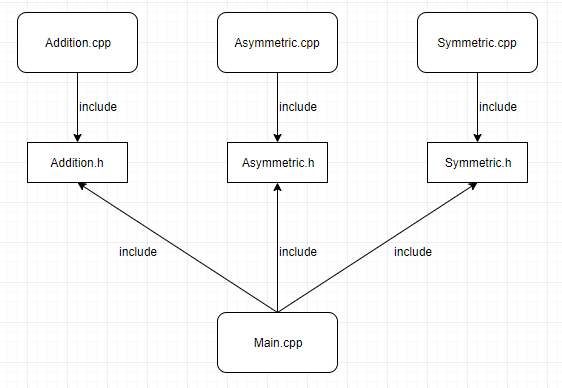
\includegraphics[scale=1]{file_structure.png}
    \caption{Các mô đun của chương trình}
    \label{fig:file_structure}
\end{figure}
Chương trình gồm 5 mô đun chính là:
\begin{itemize}
    \item Symmetric: Chứa các hàm mã hóa đối xứng tập tin sử dụng giải thuật DES.
    \item Asymmetric: Chứa các hàm mã hóa bất đối xứng tập tin sử dụng giải thuật RSA.
    \item Addition: Chứa các hàm mã hóa tập tin sử dụng kỹ thuật giấu tin (Steganography).
    \item MD5: Hàm MD5 sử dụng cho việc so sánh hai tệp.
    \item Main: Đọc các đối số và gọi các hàm phù hợp trong bốn thư viện trên.
\end{itemize}
	\subsection{Symmetric}
	Giải thuật mã hóa đối xứng nhóm sử dụng là DES với ECB mode. Trong tệp "Symmetric.h":\\
	\begin{lstlisting}[language=C]
char *stringFromFile(char filename[], const char type[]);
	\end{lstlisting}
	Trả về chuỗi giá trị trong tệp filename.\\
	type: chế độ đọc tệp ("r", "rb", ....).\\
	Lưu ý: Cần giải phóng vùng nhớ cho con trỏ trả về do có sử dụng malloc trong hàm này.\\

	\begin{lstlisting}[language=C]
unsigned char *DES_encrypt(EVP_CIPHER_CTX *en, unsigned char *plaintext, int *plain_len);
	\end{lstlisting}
	Mã hó plaintext với độ dài plain\_len theo giải thuật được quy định trong (*en).
	Trả về giá trị của chuỗi mã hóa.
	Lưu ý: Cần giải phóng vùng nhớ cho con trỏ trả về do có sử dụng malloc trong hàm này.\\

	\begin{lstlisting}[language=C]
char *DES_decrypt(EVP_CIPHER_CTX *de, unsigned char *ciphertext, int *cipher_len);
	\end{lstlisting}
	Ngược với hàm trên, hàm này giải mã ciphertext với độ dài cipher\_len.\\
	Giá trị của (*de) quy định giải thuật sử dụng để giải mã.\\
	Giá trị trả về là plaintext.\\
	Lưu ý: Cần giải phóng vùng nhớ cho con trỏ trả về do có sử dụng malloc trong hàm này.\\
	\subsection{Asymmetric}
	Giải thuật mã hóa bất đối xứng nhóm chọn là RSA.Trong tệp "Asymmetric.h":\\
	\begin{lstlisting}[language=C]
RSA * create_RSA(RSA *keypair, int pem_type, char *file_name);
	\end{lstlisting}
	Được sử dụng để tạo ra cặp key (private và public key) cho việc mã hóa và giải mã.\\
	Key được lưu trong tệp file\_name.\\

	\begin{lstlisting}[language=C]
int public_encrypt(int flen, unsigned char* from, unsigned char *to, RSA* key, int padding);
	\end{lstlisting}
	Sử dụng public key để mã hóa chuỗi (*from) với độ dài flen và lưu chuỗi mã hóa vào (*to).
	Trả về độ dài của chuỗi mã hóa.\\

	\begin{lstlisting}[language=C]
int private_decrypt(int flen, unsigned char* from, unsigned char *to, RSA* key, int padding);
	\end{lstlisting}
	Sử dụng private key để giải mã chuỗi (*from) với độ dài flen và lưu vào chuỗi (*to).\\
	Trả về giá trị độ dài của plaintext.

%%%%%%%%%%%%%%%%%%%%%%%%%%%%%%%%%
	\subsection{Addition}
	Giải thuật mã hóa ngoài bài giảng nhóm sử dụng là kỹ thuật che giấu tập tin. Trong tệp "Addition.h":\\
	\begin{lstlisting}[language=C]
void steganography_encode(char* inputfile, Mat image, char*outputfile);
	\end{lstlisting}
	Đọc tệp inputfile dưới dạng bit.\\
	Sử dụng phép tính "and" bit cho mỗi bit trong inputfile ứng với giá trị bit cuối trong mỗi kênh màu, pixels của ảnh image. Từ đó thu được một ảnh có sai khác rất nhỏ so với ảnh gốc.\\
	Ghi ảnh kết quả vào tệp outputfile.\\

	\begin{lstlisting}[language=C]
void steganography_decode(Mat image, char*outputfile);
	\end{lstlisting}
	Từ ảnh image, rút ra thông điệp và lưu nó vào outputfile.

	\subsection{MD5}
	Trong tệp "MD5Checksum.h":\\
	\begin{lstlisting}[language=C]
unsigned char *getMd5Hash(unsigned char *data, size_t dataLen, int *mdLen);
	\end{lstlisting}
	Trả về giá trị Md5Hash của data với độ dài dataLen và độ dài của Md5 được lưu trong mdLen.\\
	Lưu ý: Cần giải phóng vùng nhớ của con trỏ trả về.

	\subsection{Main}
	Hàm main chịu trách nhiệm đọc khác đối số khi chạy chương trình. Từ đó quyết định thực hiện giải thuật mã hóa nào. Nhóm có một số định nghĩa cho đối số đầu tiên như sau:\\
	\begin{lstlisting}[language=C]
#define SYMMETRIC_ENCODE	10
#define SYMMETRIC_DECODE	11
#define RSA_CREATE			20
#define RSA_ENCODE			21
#define RSA_DECODE			22
#define STREGAN_ENCODE		30
#define STREGAN_DECODE		31
#define MD5_CHECKSUM		40
	\end{lstlisting}
	Từ đây, với mỗi tùy chọn của đối số đầu tiên mà người dùng có thể lựa chọn tạo key, giải mã, mã hóa hay so sánh hai tệp.\\

	Ngoài ra, trong hàm main, nhóm có gọi hàm clock() trước và sau khi thực hiện chương trình để đo thời gian mã hóa và giải mã.

%%%%%%%%%%%%%%%%%%%%%%%%%%%%%%%%%
\section{Chạy thử chương trình}
	\subsection{Mã hóa DES}
    Chạy chương trình với command:\\
    \$File.exe 10 inputfile inputkeyfile outputfile\\
    Trong đó:
    \begin{itemize}
        \item File.exe : tệp thực thi được tạo từ MSVC.
        \item 10 : để lựa chọn thực thi mã hóa DES.
        \item inputfile: đường dẫn đến tệp cần mã hóa.
        \item inputkeyfile: đường dẫn đến tệp chứa key mã hóa.
        \item outputfile: đường dẫn đến tệp kết quả. 
    \end{itemize}
    
    Ví dụ hình \ref{fig:desen}
    \begin{figure}[htp]
        \centering
        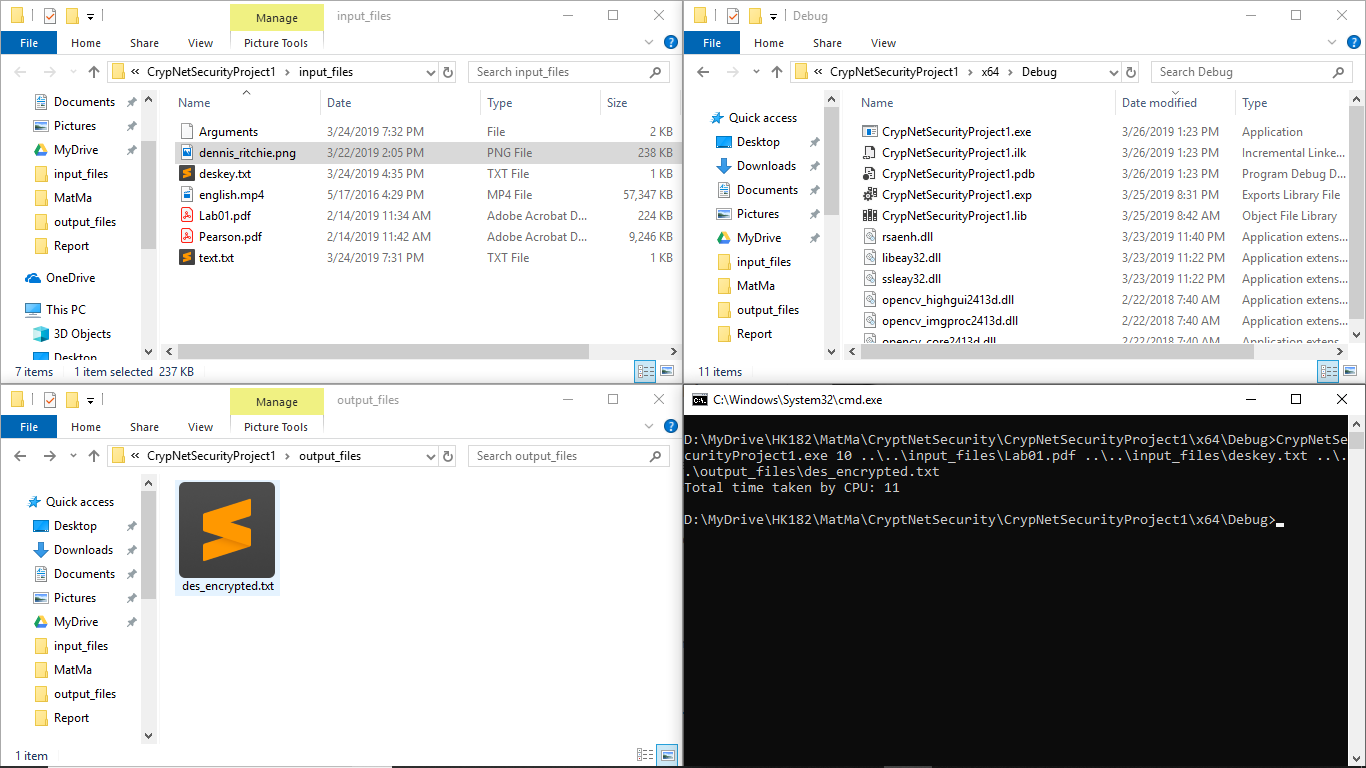
\includegraphics[scale=0.4]{desen.png}
        \caption{Mã hóa DES}
        \label{fig:desen}
    \end{figure}
	
	Từ hình \ref{fig:desen}, ta thấy mất 11ms để mã hóa tệp Lab01.pdf và tệp mã hóa (des\_encrypted.txt) được tạo.
	\subsection{Giải mã DES}
    Chạy chương trình với command:\\
    \$File.exe 11 inputkeyfile inputfile outputfile\\
    Trong đó:
    \begin{itemize}
        \item File.exe : tệp thực thi được tạo từ MSVC.
        \item 11 : để lựa chọn thực thi giải mã DES.
        \item inputfile: đường dẫn đến tệp cần giải mã.
        \item inputkeyfile: đường dẫn đến tệp chứa key mã hóa.
        \item outputfile: đường dẫn đến tệp kết quả. 
    \end{itemize}

    Ví dụ hình \ref{fig:desde}
    \begin{figure}[htp]
        \centering
        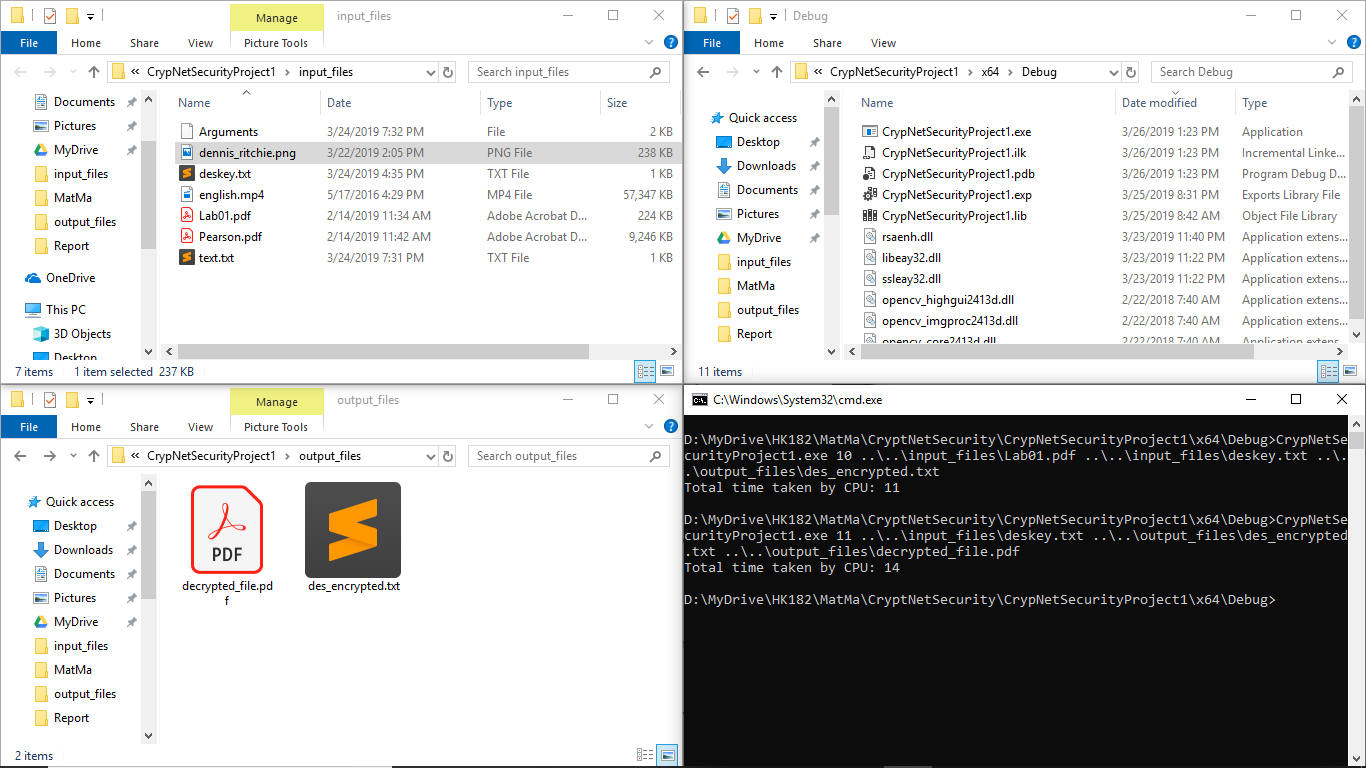
\includegraphics[scale=0.4]{desde.png}
        \caption{Giải mã DES}
        \label{fig:desde}
    \end{figure}
    Từ hình \ref{fig:desde}, ta thấy tệp des\_encrypted.txt được giải mã trong vòng 14ms và tạo ra tệp giải mã decrypted\_file.pdf.
    \begin{figure}[htp]
        \centering
        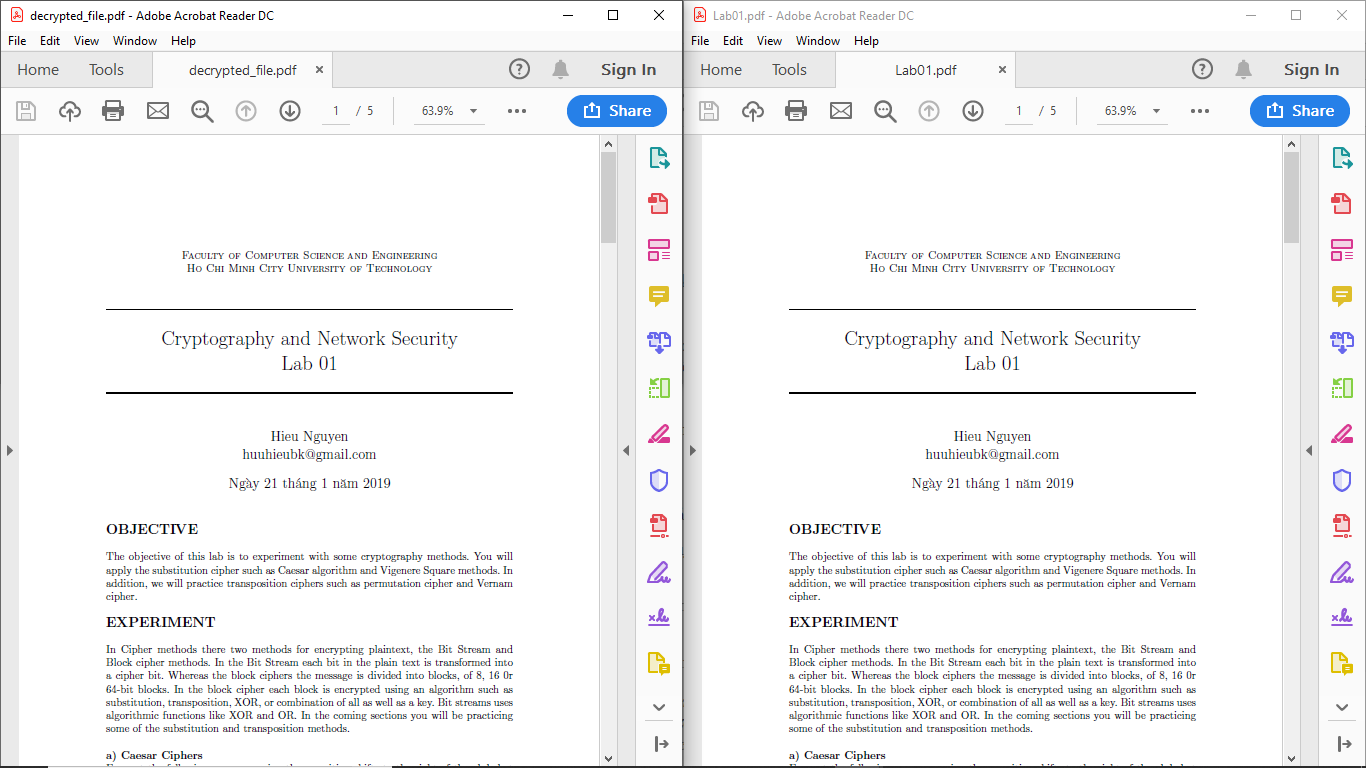
\includegraphics[scale=0.4]{descmp.png}
        \caption{Kết quả của giải thuật DES}
        \label{fig:descmp}
    \end{figure}
    Kết quả của giải thuật DES đã tạo ra tệp giải mã và được miêu tả ngắn gọn trong hình \ref{fig:descmp}.

    \subsection{Tạo khóa RSA}
    Chạy chương trình với command:\\
    \$File.exe 20  privateouput publicoutput\\
    Trong đó:
    \begin{itemize}
        \item File.exe : tệp thực thi được tạo từ MSVC.
        \item 20 : để lựa chọn thực thi tạo khóa bí mật và công khai.
        \item privateouput: đường dẫn đến tệp chứa khóa bí mật.
        \item publicoutput: đường dẫn đến tệp chứa khóa công khai.
        \item outputfile: đường dẫn đến tệp kết quả. 
    \end{itemize}
    Ví dụ hình \ref{fig:rsacreate}. Mất 418ms để tạo ra cặp khóa bí mật và công khai. Hai khóa trên ghi vào hai tệp: private\_key.pem và  public\_key.pem.
    \begin{figure}[htp]
        \centering
        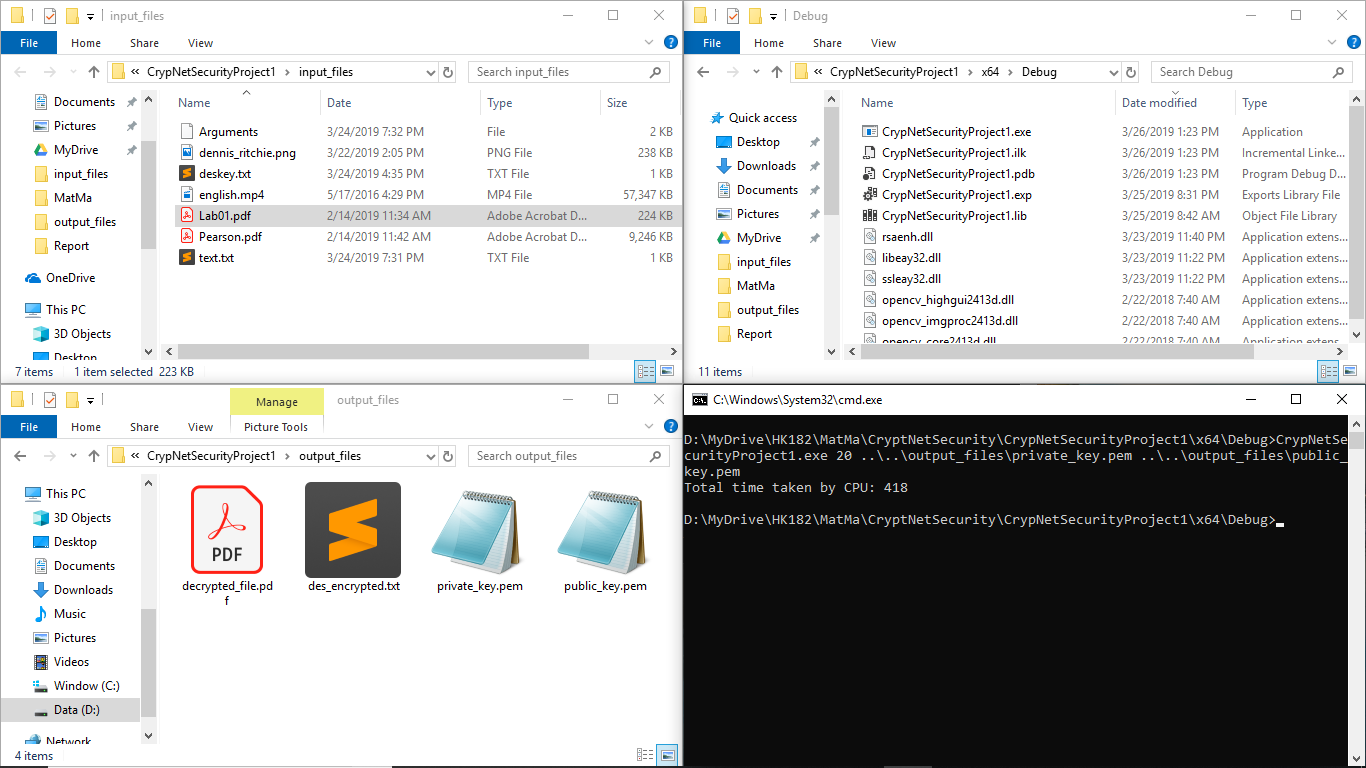
\includegraphics[scale=0.4]{rsacreate.png}
        \caption{Tạo cặp khóa công khai và bí mật}
        \label{fig:rsacreate}
    \end{figure}
    \subsection{Mã hóa RSA}
    Chạy chương trình với command:\\
    \$File.exe 21 inputfile  privateouput publicoutput outputfile\\
    Trong đó:
    \begin{itemize}
        \item File.exe : tệp thực thi được tạo từ MSVC.
        \item 21 : để lựa chọn thực thi tạo khóa bí mật và công khai.
        \item inputfile: đường dẫn đến tệp cần mã hóa.
        \item privateouput: đường dẫn đến tệp chứa khóa bí mật.
        \item publicoutput: đường dẫn đến tệp chứa khóa công khai.
    \end{itemize}
    Ví dụ hình \ref{fig:rsaen}. Mất 183ms để mã hóa tệp text.txt. Kết quả mã hóa được ghi xuống tệp encrypted\_file.bin
    \begin{figure}[htp]
        \centering
        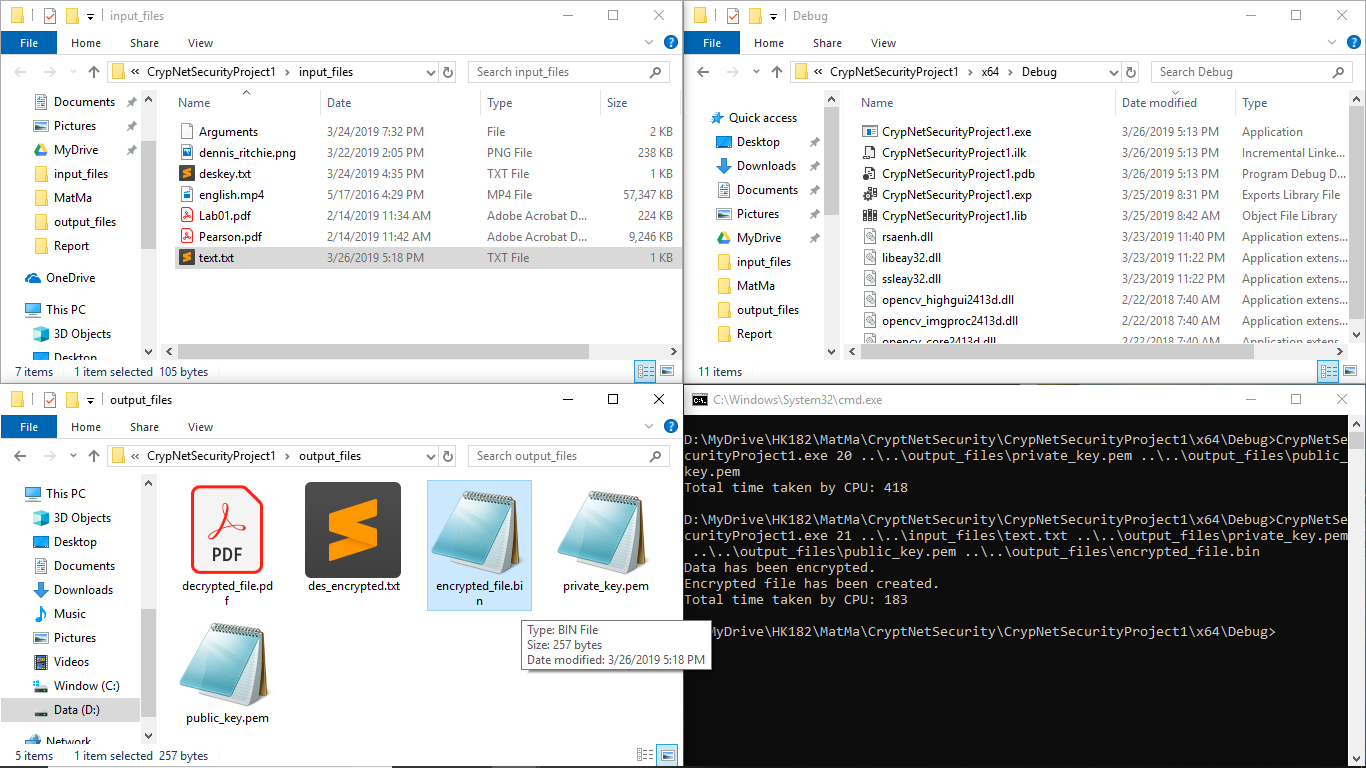
\includegraphics[scale=0.4]{rsaen.png}
        \caption{Tạo cặp khóa công khai và bí mật}
        \label{fig:rsaen}
    \end{figure}
    \subsection{Giải mã RSA}
    Chạy chương trình với command:\\
    \$File.exe 22 privateinput inputfile outputfile\\
    Trong đó:
    \begin{itemize}
        \item File.exe : tệp thực thi được tạo từ MSVC.
        \item 22 : để lựa chọn thực thi mã hóa tệp theo giải thuật RSA.
        \item privateinput: đường dẫn đến tệp chứa khóa bí mật.
        \item inputfile: đường dẫn đến tệp cần giải mã.
        \item outputfile: đường dẫn đến tệp kết quả của phép giải mã.
    \end{itemize}
    Ví dụ hình \ref{fig:rsade}. Mất 155ms để giải mã tệp encrypted\_file.bin. Kết quả mã hóa được ghi xuống tệp decrypted\_file.txt.\\
    \begin{figure}[htp]
        \centering
        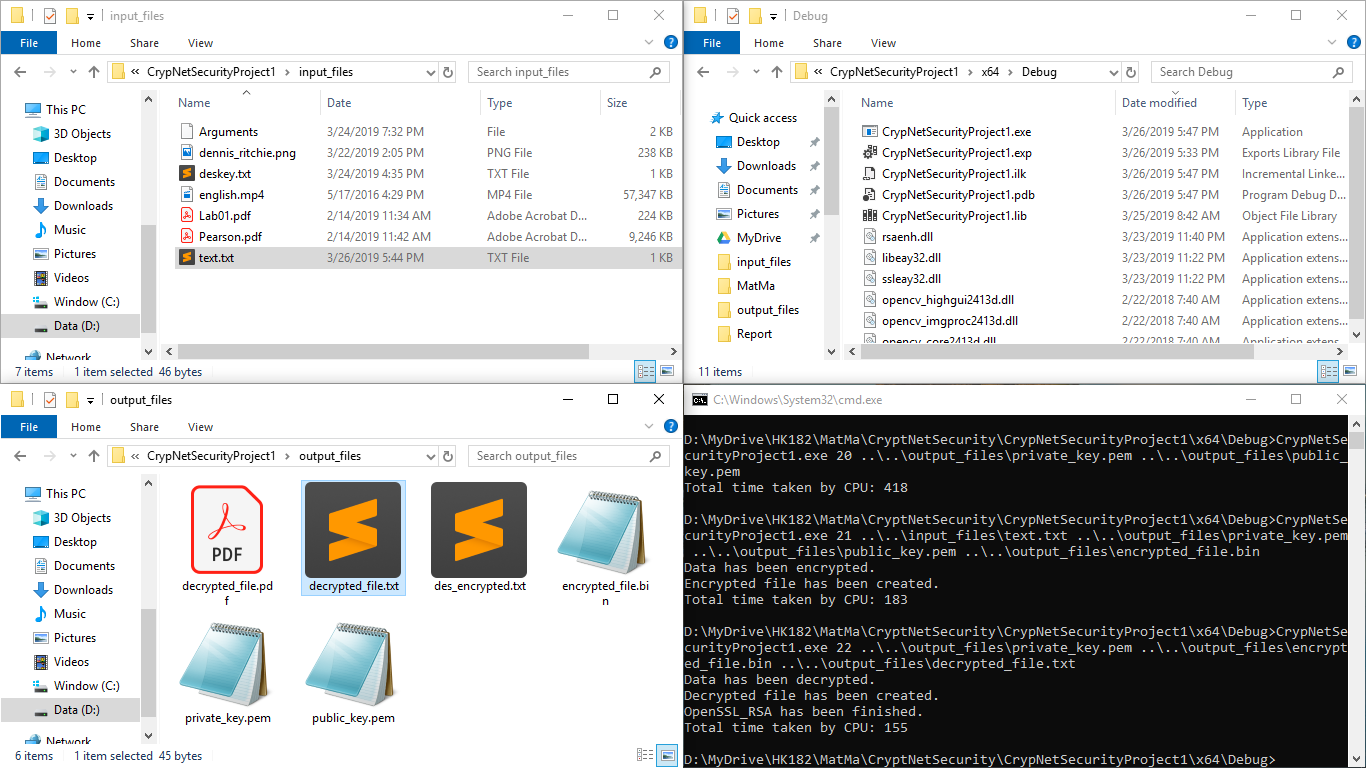
\includegraphics[scale=0.4]{rsade.png}
        \caption{Tạo cặp khóa công khai và bí mật}
        \label{fig:rsade}
    \end{figure}
    Hình \ref{fig:rsacmp} thể hiện trực quan so sánh giữa tệp ban đầu và tệp sau mã hóa.
    \begin{figure}[htp]
        \centering
        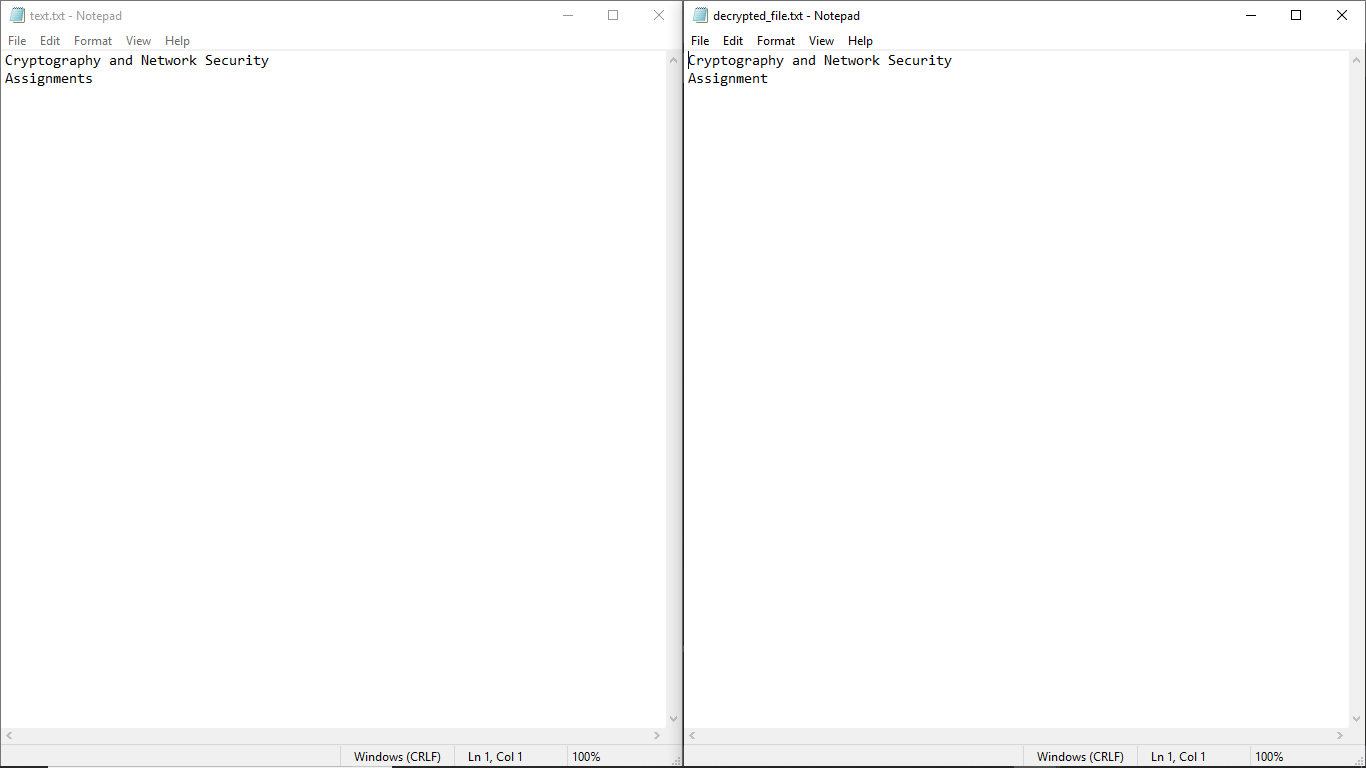
\includegraphics[scale=0.4]{rsacmp.png}
        \caption{Tạo cặp khóa công khai và bí mật}
        \label{fig:rsacmp}
    \end{figure}
    \subsection{Kỹ thuật giấu tin}
    Chạy chương trình với command sau để gắn thông điệp vào ảnh mang:\\
    \$File.exe 30 inputfile1 inputfile2 outputfile\\
    Trong đó:
    \begin{itemize}
        \item File.exe : tệp thực thi được tạo từ MSVC.
        \item inputfile1: đường dẫn đến tệp chứa thông điệp.
        \item inputfile2: đường dẫn đến tệp chứa ảnh mang.
        \item outputfile: đường dẫn đến tệp kết quả của phép giấu tin.
    \end{itemize}
    Ví dụ hình \ref{fig:steen}
    \begin{figure}[htp]
        \centering
        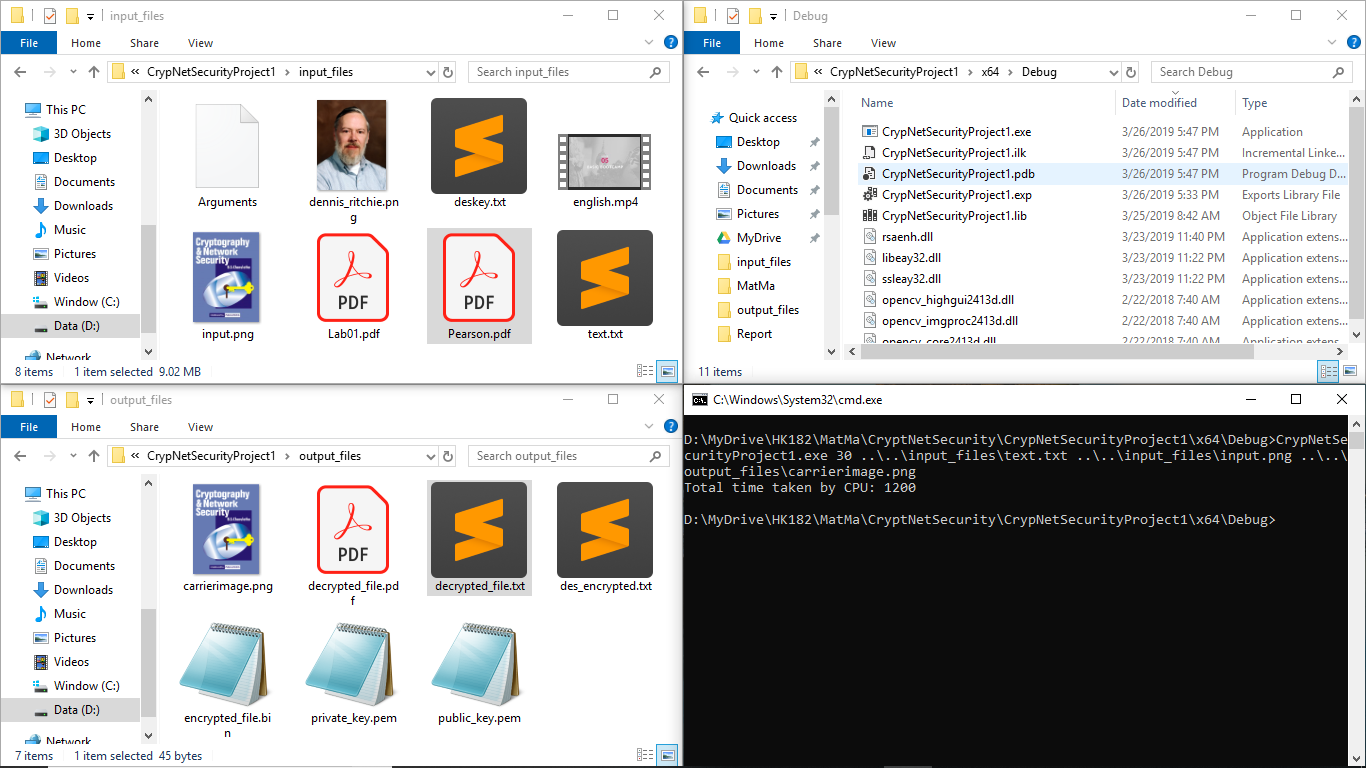
\includegraphics[scale=0.4]{steen.png}
        \caption{Gắn thông điệp vào ảnh mang}
        \label{fig:steen}
    \end{figure}

    Chạy chương trình với command sau để gắn thông điệp vào ảnh mang:\\
    \$File.exe 30 inputfile outputfile\\
    Trong đó:
    \begin{itemize}
        \item File.exe : tệp thực thi được tạo từ MSVC.
        \item inputfile: đường dẫn đến tệp chứa ảnh mang thông điệp.
        \item outputfile: đường dẫn đến tệp giải mã.
    \end{itemize}
    Ví dụ hình \ref{fig:stede}
    \begin{figure}[htp]
        \centering
        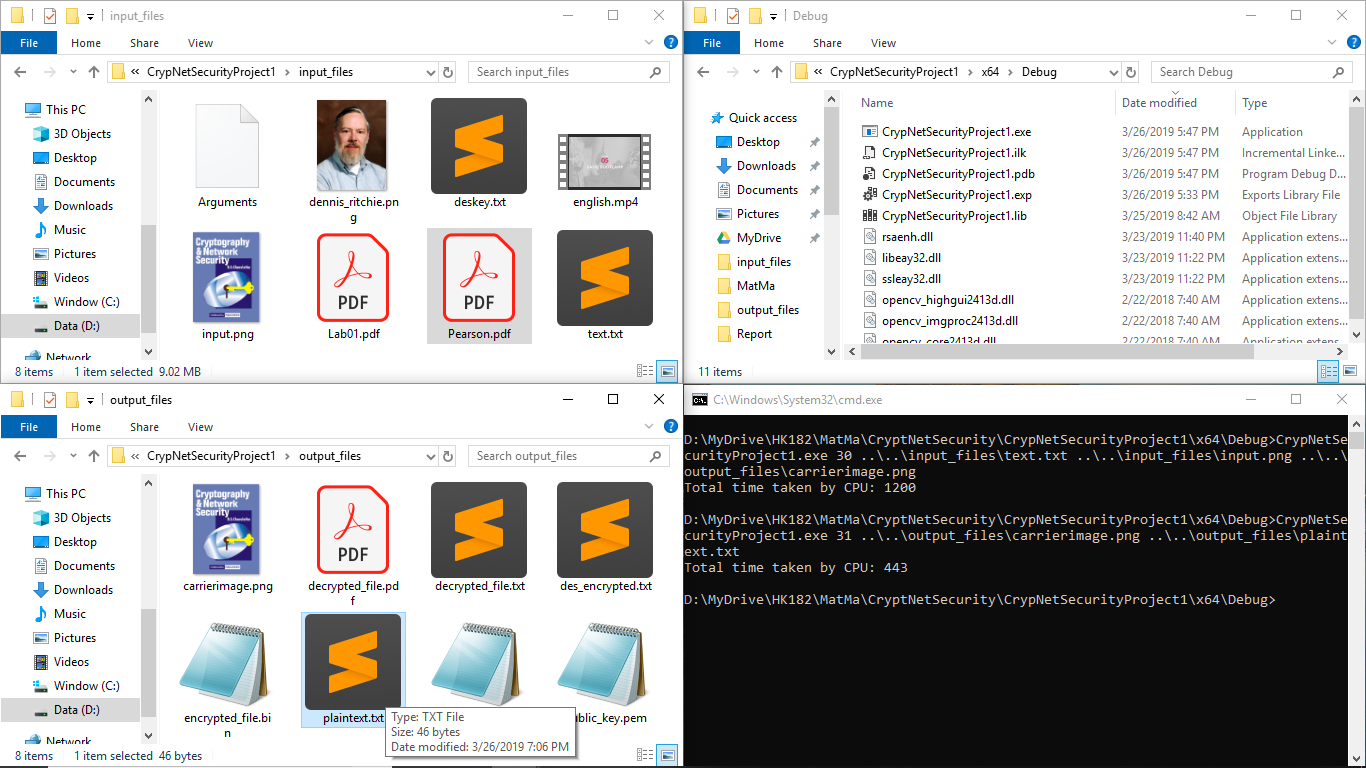
\includegraphics[scale=0.4]{stede.png}
        \caption{Lấy thông điệp từ ảnh mang}
        \label{fig:stede}
    \end{figure}

    Kết quả của quá trình giải mã và mã hóa được thể hiện qua hình \ref{fig:stecmp}
    \begin{figure}[htp]
        \centering
        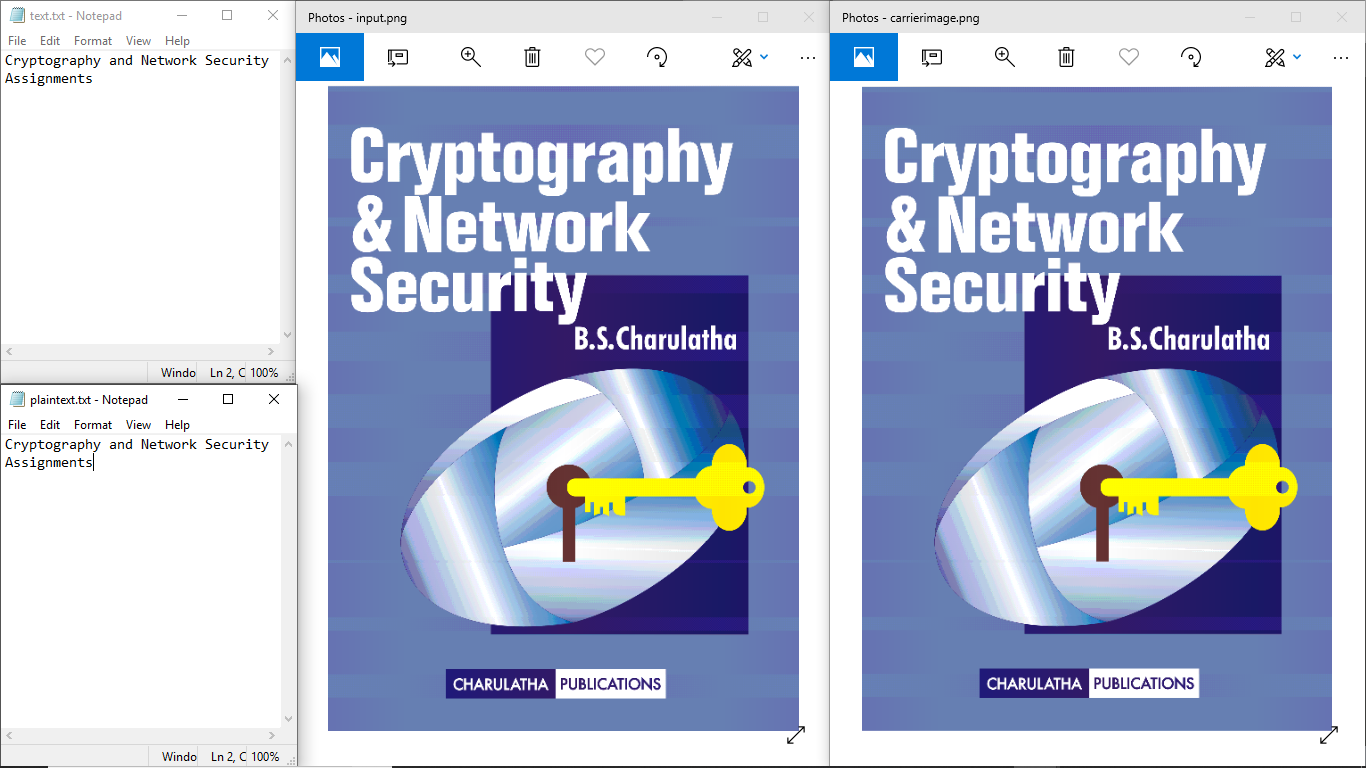
\includegraphics[scale=0.4]{stecmp.png}
        \caption{So sánh input và output của kỹ thuật giấu tin}
        \label{fig:stecmp}
    \end{figure}
%%%%%%%%%%%%%%%%%%%%%%%%%%%%%%%%%
\section{Hướng dẫn vận hành trên MSVC}
	Bước 1: Cài đặt MSVC.\\
    Bước 2: Cài đặt opencv.\\
    Bước 3: Cài đặt opensll.\\
    Bước 4: Tạo project trên MSVC.\\
    Bước 5: Thiết lập đường dẫn đến thư viện opencv và openssl như hình \ref{fig:msvcinclude} \ref{fig:msvclib} và \ref{fig:msvcinput}\\
    Bước 6: Tải mã nguồn tại url{https://github.com/nxnam714/CryptNetSecurity.git} và gom vào project.
    \begin{figure}[htp]
        \centering
        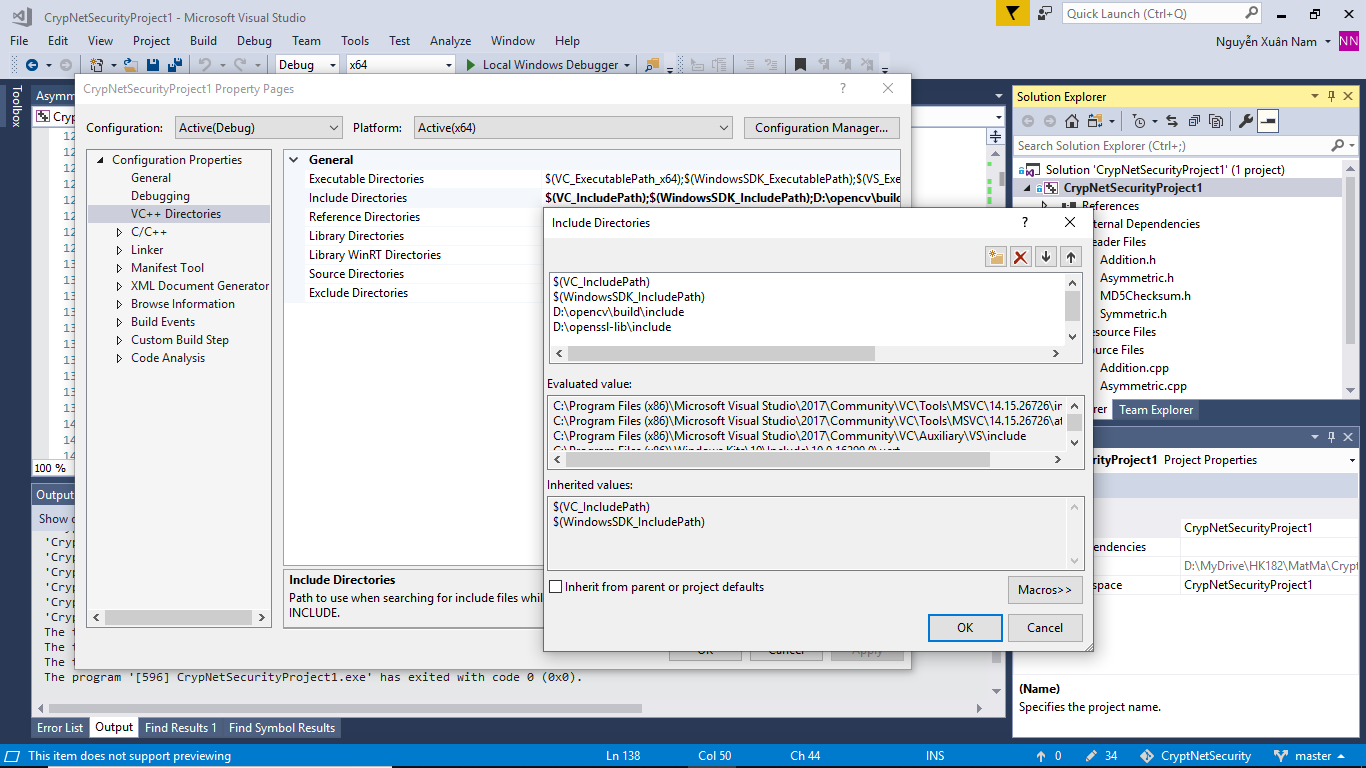
\includegraphics[scale=0.4]{msvcinclude.png}
        \caption{Lấy thông điệp từ ảnh mang}
        \label{fig:msvcinclude}
    \end{figure}
    \begin{figure}[htp]
        \centering
        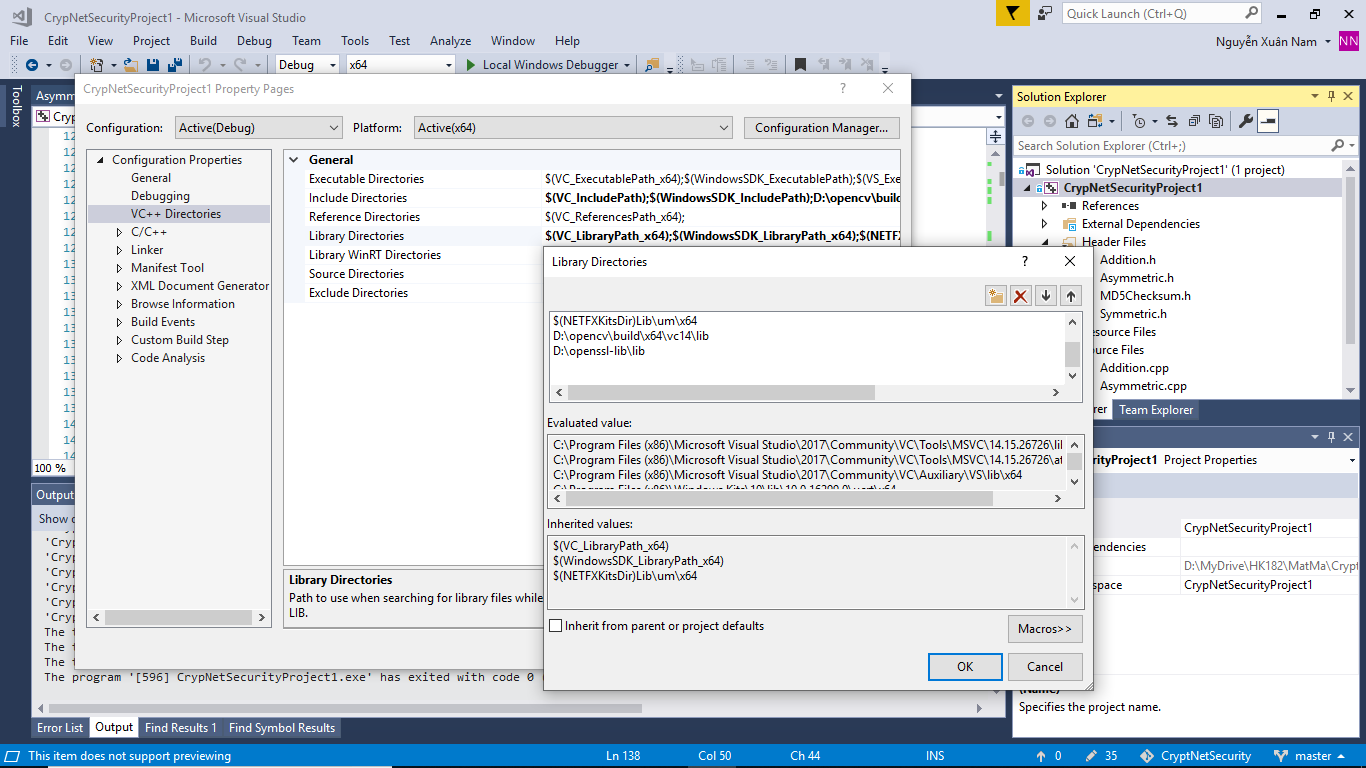
\includegraphics[scale=0.4]{msvclib.png}
        \caption{Lấy thông điệp từ ảnh mang}
        \label{fig:msvclib}
    \end{figure}
    \begin{figure}[htp]
        \centering
        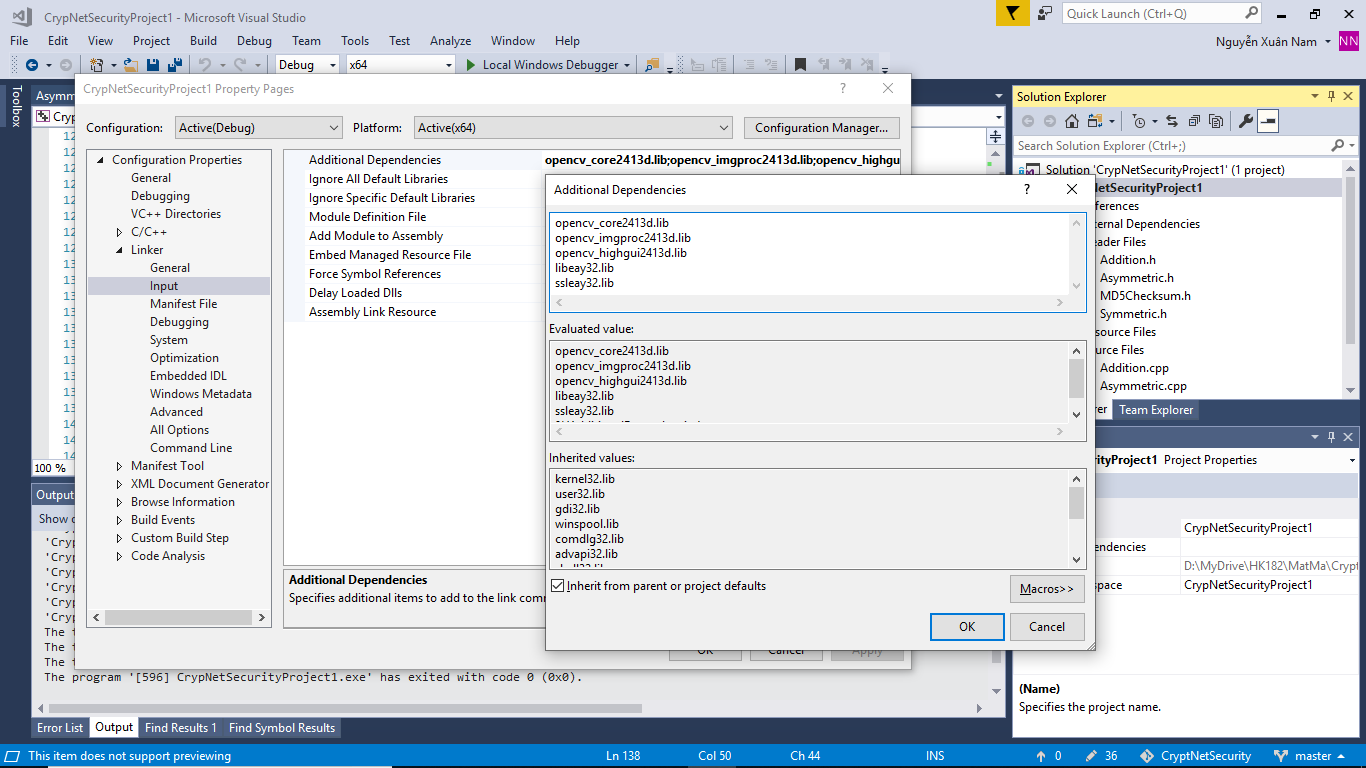
\includegraphics[scale=0.4]{msvcinput.png}
        \caption{Lấy thông điệp từ ảnh mang}
        \label{fig:msvcinput}
    \end{figure}
%%%%%%%%%%%%%%%%%%%%%%%%%%%%%%%%%
\section{Phân tích và kết luận}
Ứng dụng có thể chạy tốt ba giải thuật mã hóa.
\begin{itemize}
    \item Kết quả giải mã là đồng nhất với dữ liệu đưa vào dựa vào hàm kiểm tra MD5.
    \item Có thể mã hóa các tệp cơ bản như pdf, png, txt,...
    \item Thời gian thực thi nhanh.
\end{itemize}
Tuy nhiên còn một số khuyết điểm:
\begin{itemize}
    \item Tính thực tế của ứng dụng chưa cao, chỉ có thể sử dụng cho việc mã hóa các tệp trong máy. Đồng thời việc bảo khóa bí mật chưa được quan tâm đến.
    \item Ứng dụng không có giao diện nên tạo khó khăn cho việc sử dụng.
    \item Không có thanh trạng thái báo cho người dùng biết quá trình mã hóa đang diễn ra.
\end{itemize}
Hướng phát triển ứng dụng:
\begin{itemize}
    \item Khắc phục các nhược điểm được nêu ra.
    \item Kết hợp các giải thuật mã hóa đã hiện thực để tao ứng dụng nhắn tin an toàn.
\end{itemize}
%%%%%%%%%%%%%%%%%%%%%%%%%%%%%%%%%
\section{Phân công công việc}
Khối lượng công việc được chia đều cho các thành viên trong nhóm như sau:
\begin{itemize}
    \item Nguyễn Trần Lê Minh: Hiện thực khối DES.
    \item Lê Duy Thanh: Hiện thực khối RSA.
    \item Nguyễn Xuân Nam: Hiện thực khối MD5 và Steganography.
\end{itemize}

%%%%%%%%%%%%%%%%%%%%%%%%%%%%%%%%%
\newpage
\begin{thebibliography}{80}


\bibitem{openssl}
Thư viện openssl, \url{https://www.openssl.org/docs/man1.0.2/}


\bibitem{book}
Sách giáo khoa môn học: Stallings, William - Cryptography and network security principles and practice (2017, Pearson).


\end{thebibliography}
\end{document}

